\documentclass[como,a4paper,12pt,final]{Classes/c4e-preprint}
\graphicspath{{Figures/}}

%--------------------------------------------------------------------
%    LaTeX includes
%--------------------------------------------------------------------
% Note subfig is now deprecated.
\usepackage{subfig}
\usepackage{graphicx}
\usepackage{xspace}

%--------------------------------------------------------------------
%    pdf properties (must be consistent with title page data below)
%--------------------------------------------------------------------
\hypersetup{
  pdftitle={Structure and properties of curved polycyclic aromatic hydrocarbon nanoclusters},
  pdfauthor={Kimberly Bowal\affiliated{1}, Laura Pascazio\affiliated{1}, Jacob W. Martin\affiliated{1,2}, Markus Kraft\affiliated{1,2,3}}
  pdfsubject={c4e preprint template},
  pdfkeywords={c4e, preprint, template}
  }

\begin{document}
%--------------------------------------------------------------------
%    title page (must be consistent with pdf properties above)
%--------------------------------------------------------------------
\title{Structure and properties of curved polycyclic aromatic hydrocarbon nanoclusters}
\author{Kimberly Bowal\affiliated{1}, Laura Pascazio\affiliated{1}, Jacob W. Martin\affiliated{1,2}, Markus Kraft\affiliated{1,2,3}}
\keywords{force field, curved polycyclic aromatic hydrocarbon, flexoelectric dipole, ion-induced nucleation, soot formation}
\nopreprint{XXX} \nopreyear{2019} \releasedate{XXX}

\affiliation{1}{
  Department of Chemical Engineering \\and Biotechnology\\
  University of Cambridge\\
  West Site, Philippa Fawcett Drive\\
  Cambridge, CB3 0AS\\
  United Kingdom\\
E-mail: \href{mailto:mk306@cam.ac.uk}{mk306@cam.ac.uk}}
  
\affiliation{2}{
  Cambridge Centre for Advanced Research\\
  and Education in Singapore (CARES)\\
  CREATE Tower, 1 Create Way\\
  Singapore, 138602}

\affiliation{3}{
  School of Chemical and\\ Biomedical Engineering\\
  Nanyang Technological University\\
  62 Nanyang Drive\\
  Singapore, 637459}



\maketitle

%--------------------------------------------------------------------
%     abstract
%--------------------------------------------------------------------
\begin{abstract}
Understanding the formation and properties of soot particles is critical for the accurate description of turbulent reacting flows within combustion. Due to the small time and length scale of these particle dynamics, a complete description of soot particle properties has remained a challenge. Curved polycyclic aromatic hydrocarbons (cPAHs) have been identified as key constituents of soot particles and we have recently shown that their interactions with ions may contribute significantly to particle formation (Bowal, K, et al. “Ion-induced soot nucleation using a new potential for curved aromatics”, Combustion Science and Technology (2018, accepted)). The structural properties of cPAH clusters are unknown and further molecular modelling studies are required to provide insight into the clustering behaviour of cPAHs - their size-dependent arrangements, interactions with planar PAHs, and assembly around ions.

\end{abstract}

%%\begin{figure}[!ht]
%%    \setlength{\figwidth}{12cm}
%%    \centering
%%    \resizebox*{\figwidth}{!}{\includegraphics{GraphicalAbstract.pdf}}
%%\end{figure}

\textbf{Highlights:}
\begin{itemize}
\item item 1
\item item 2
\end{itemize}

\vfill

%--------------------------------------------------------------------
%     table of contents
%--------------------------------------------------------------------
\clearpage \setcounter{tocdepth}{3} \tableofcontents

%--------------------------------------------------------------------
%     paper body
%--------------------------------------------------------------------
\clearpage
%use input{} to include the body of the preprint
\newcommand{\curPAHAP}{curPAHIP\xspace} 
%
\section{Introduction}
\label{sec:Introduction}
% 
%% Curved carbons are found in porous carbons, glassy carbons, soot, etc


%% Curvature is caused by non-hexagonal rings, causes special steric and electronic properties


%% Curved carbons have great promise in many applications such as understanding particulates, novel nanocarbon materials, batteries, drug delivery, sensors, gas storage, etc
Preliminary simulations show that cluster arrangment of curved corannulene is different than planar coronene (Preprint 214). This may be more representative of the experimentally observed structure of nascent soot particles.

Further areas of interest include: arrangement of curved and planar PAH clusters, structure of cPAH clusters containing ion(s)

The structural properties of cPAH clusters are unknown and further molecular modelling studies are required to provide insight into the clustering behaviour of cPAHs - their size-dependent arrangements, interactions with planar PAHs, and assembly around ions.

Understanding non-covalent interactions with and between curved carbon nanostructures has importance in many systems and great potential for numerous applications.

Motivation: structure of soot particles / interstellar medium, applications such as electronics, nanomedicine, energy, etc



%% Previous work looking at cPAH interactions:	Homogeneous dimers
Significant energy between nested concave-to-convex cPAHs so curvature doesn’t prevent dimers from forming pi-pi stacked assemblies similar to planar systems (10.1002/qua.21794). Curvature increases interaction strength by decreasing C-C distances for increased dispersion interactions (10.1021/jp305700k). Very curved PAHs may have interaction strengths similar to fPAHs though because of increased sterics (10.1016/j.proci.2018.05.046, 10.1002/qua.21794?

As with fPAHs, cPAH dimer interactions are dominated by $\pi$-$\pi$ interactions compared to the CH-$\pi$ interactions. However cPAHs show different behaviour than fPAHs, with eclipsed dimer showing more stability than the staggered dimer (10.1016/j.cplett.2011.07.030).



%% Previous work looking at cPAH interactions:	Bulk systems
Corannulene has no long-range stacked order in crystal analysis  - CH-pi interactions dominate (10.1107/S0567740876012430)
cPAHs with increased curvature and rigidity and heteroatoms form columnar stacks (many refs, including 10.1021/cg100898g)
Condensed / larger systems: pi-H stacking in crystal (10.1515/znb-2010-0403) 

So expect homogeneous corannulene nanocluster to be disordered, homo 2pent15ring cluster to have stacks

Mixed cluster – expect to be dominated by 2pent15rings but enhanced corannulene stacking.


%% Previous work looking at cPAH interactions:	Heterogeneous systems (dimers, etc)
Planar PAH studies show that heterogeneity decreases the stability of the nanocluster since heterogeneous dimers are significantly weaker.  This leads to a distinct partitioning 

something about cPAH hetero dimers/systems...

Thus we hypothesise that heterogeneous cPAH clusters may be more stable than their heterogeneous fPAH counterparts since different sizes of cPAHs may provide stable packing arrangements.


%% Limitations: mostly static DFT calculations, no information about nanoparticles. 



%% Following previous work looking at heterogeneous fPAHs…
Previous work examined heterogeneous PAH clusters using replica exchange molecular dynamics (ref)...

%% 
The purpose of this work is to explore properties (molecular arrangements, melting points, densities, surface properties, etc) of clusters containing curved PAHs.  
Hypothesis: cPAH clusters are more representative of the experimentally observed structure of nascent soot particles, heterogeneous cPAH clusters are significant since they are stable than their fPAH counterparts.
This is important for better understanding of soot particle formation and growth, and has implications for other carbon nanomaterials such as ???

%
\section{Conclusions}


\section*{Acknowledgements}
This work used the ARCHER UK National Supercomputing Service (\url{http://www.archer.ac.uk}).
K.B. is grateful to the Cambridge Trust and the Stanley Studentship at King's College, Cambridge for their financial support.
This project is also supported by the National Research Foundation (NRF), Prime Minister's Office, Singapore under its Campus for Research Excellence and Technological Enterprise (CREATE) programme.


%--------------------------------------------------------------------
%     appendices
%--------------------------------------------------------------------
\clearpage \appendix
\numberwithin{equation}{section}
%\beginsupplement
\section{Supplementary Data}
\label{supplinfo}


\subsection{Potentials}
isoPAHAP tables?
curPAHIP tables?

The atomic coordinates and charges of the minimised 2pent15ring monomer.
Probably should also include the same for corannulene (can pull from CST paper).

\subsection{Dimer energy plots - isoPAHAP potential}

\subsection{Position restraint neglibigility at low temperature}

\subsection{Simulation length equilibration check}
Energies and radial distances don't change significantly when comparing eqm result from 3ns simulation (final 1ns) or 1ns simulation (final 500ps)
Percent error of intermolecular energies are less than 0.2\%
Percent error of radial distances are less than 3.5\%



\subsection{Corannulene crystal structure}
In order to assess / benchmark the structural metrics used in this paper, they have been applied to the known crystal structure of a corannulene. %Further comparison is made with a 2pent15ring system and published large cPAH systems - Actually this should be included in the discussion sections of the paper I think.

X-ray analysis of corannulene was conducted in 1975, and it was determined that the compound crystallises in space group \textit{P}$2_{1}/c$ \cite{hanson1976crystal}.

A crystal structure containing 18 molecules, taken from The Cambridge Crystallographic Data Centre \cite{CORANN11unitcell}, provides an independent verification of the analysis used in this work as well as a known experimental structure useful for comparison.  The crystal density and intermolecular distances are provided in Table \ref{table:crystal}.  Figure XX shows the crystal structure and alignment angles.

% Please add the following required packages to your document preamble:
% \usepackage{multirow}
\begin{table}[]
\centering
\caption{Molecular configuration metrics of corannulene crystal structure (collected from \cite{CORANN11unitcell}).}
\label{table:crystal}
\begin{tabular}{cc|cll}
\multicolumn{2}{c}{Density (kg/m3)} & 1.36 \cite{CORANN11unitcell}&  &  \\ \cline{1-3}
\multirow{3}{*}{Average intermolecular distance (nm)} & 1 molecule & 0.57 &  &  \\
 & 2 molecule & 0.72 &  &  \\
 & 3 molecule & 0.76 &  &  \\ \cline{1-3}
\multirow{3}{*}{Intermolecular distances (nm)} & 1 molecule & 0.55 x 10, 0.61 x 6 &  &  \\
 & 2 molecules & 0.61 x 2, 0.72 x 10, 0.73 x 2, 0.76 x 2, 0.78 x 2 &  &  \\
 & 3 molecules & 0.72 x 2, 0.73 x 4, 0.76 x 8, 0.78 x 2, 0.82 x 2 &  & 
\end{tabular}
\end{table}
%
%(using cut-off value of $R = 0.7$ nm)
%Intermolecular distances: 0.55 nm x 10, 0.61 nm x 6 (for first molecule); 0.61 x 2, 0.72 x 10, 0.73 x 2, 0.76 x 2, 0.78 x 2 (for second molecule), 0.72 x 2, 0.73 x 4, 0.76 x 8, 0.78 x 2, 0.82 x 2 (third molecule)... NOT SURE HOW TO SHOW THESE -> FOLLOW SAME PATTERN USED IN HOW I DISCUSS THIS IN THE PAPER (AVERAGE INTERMOLECULAR DISTS? - WOULD BE 0.57 NM FOR FIRST MOLECULE, ETC)
%
\begin{figure}[!tbh]
\centering
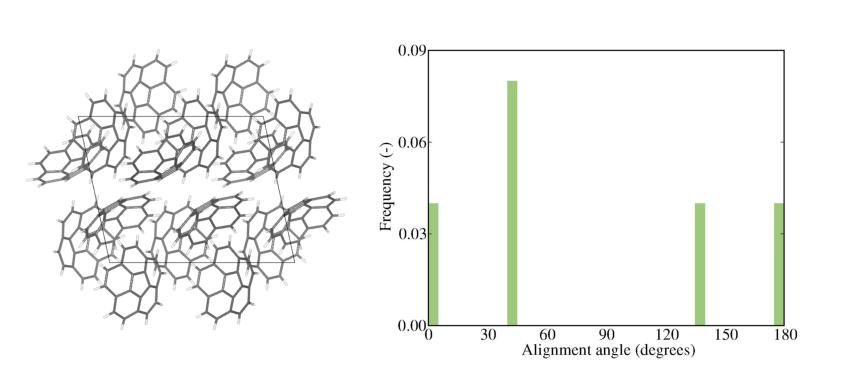
\includegraphics[width=0.65\linewidth]{Figures/corannulene_crystal.eps}
\caption{Snapshot of corannulene crystal structure (left) with alignment angle distribution (right).}
\label{fig:corannulene_crystal}
\end{figure}
%

\subsection{Cut-off distance sensitivities}
The selection of the cut-off distance, $R$, influences the calculated average intermolecular distances, coordination numbers, and alignment angles.

Due to the molecular arrangements of the homogeneous corannulene clusters (that is, sandwich-type stacking is not present), these results are the most sensitive to the selection of $R$.

- Include figure of CN histograms with r=0.5 for corannulene and 2pent15ring

- Include figures of alignment angles using R=0.5, 0.6, 0.7, 0.8 for a representative system (ann\_25?)

Note that for all systems, no neighbouring molecules are found using a cut-off distance of 0.400 nm or smaller.

\newpage

%--------------------------------------------------------------------
%     bibliography
%--------------------------------------------------------------------
\clearpage \citeindexfalse
\bibliography{c4e-preprint-bibliography}    %Create bibliography
%GATHER{c4e-preprint-bibliography.bib}      %Get WinEdt data

%--------------------------------------------------------------------
%     citation index
%--------------------------------------------------------------------
%\clearpage \makeciteindex

\end{document}
